\section{Waveforms}
We will now comment some of the observed waveforms of the simulation of our hardware module.

As reported in \cref{sec:usage}, the module shall be reset at startup. On reset, we can observe that the \lstinline{dout_valid} signal is set to zero.
We wait for the posedge of the \lstinline{rst_n} signal to start the simulation, which starts by loading the key. We can also observe that each cycle an input is fed, and the corresponding output is available at the next clock cycle, as per specification.
\begin{figure}[!ht]
    \centering
    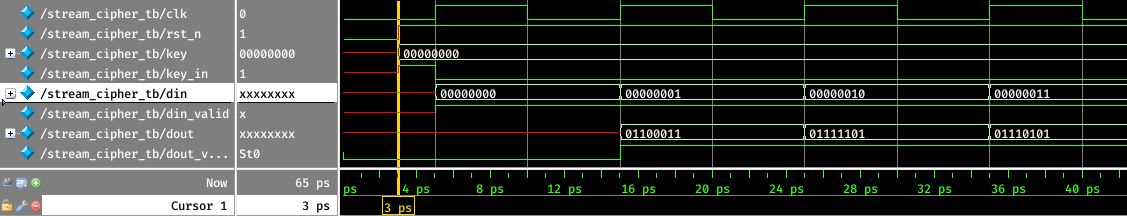
\includegraphics[width=1\textwidth]{startup_waveform}
    \caption{Startup waveform}
    \label{fig:startup_waveform}
\end{figure}

The following is the waveform for a key change. Note that in the cycle next to the key change there is no output, therefore \lstinline{dout_valid} will always be deasserted.
\begin{figure}[!ht]
    \centering
    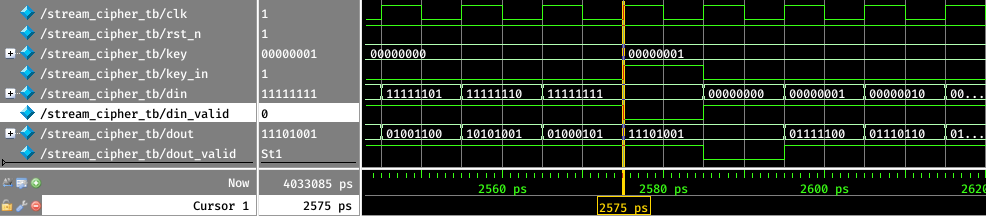
\includegraphics[width=1\textwidth]{key_change}
    \caption{Key change}
    \label{fig:key_change}
\end{figure}

Here we report the waveform of the \nth{2} test (see \cref{sec:tests}). We can observe that, independently from the number of clock cycles the module waits, signals follow the specification.
\begin{figure}[!ht]
    \centering
    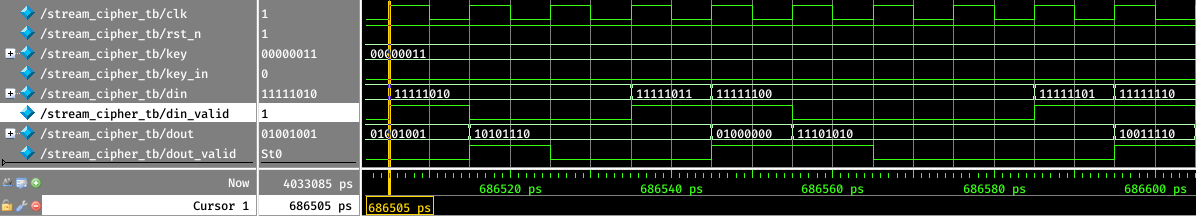
\includegraphics[width=1\textwidth]{random_waveform}
    \caption{Encryption waiting a random number of clock cycles}
    \label{fig:random_waveform}
\end{figure}

\clearpage
Finally, here we report the waveform of the \nth{3} test (see \cref{sec:tests}).
\begin{figure}[!ht]
    \centering
    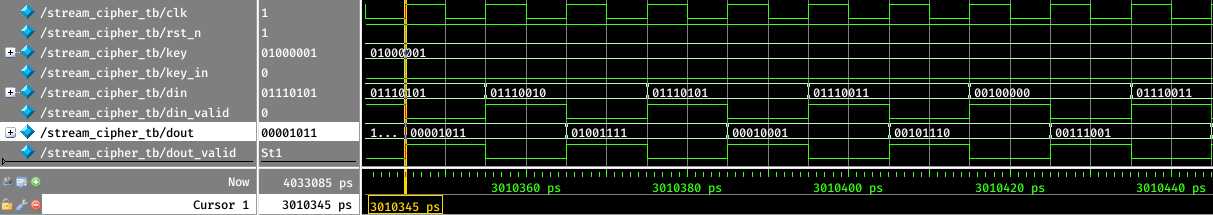
\includegraphics[width=1\textwidth]{file_encryption}
    \caption{File encryption/decryption waveform}
    \label{fig:file_encryption}
\end{figure}